\documentclass[11pt]{article}

% ---------------------------------------------------------------
% Neutral preprint style (no venue branding).
% Compiles with pdflatex; falls back cleanly if a package is missing.
% Style reference: gssm.tex (same document class, macros, citation style).
% ---------------------------------------------------------------
\usepackage[utf8]{inputenc}
\usepackage[T1]{fontenc}
\usepackage[margin=1in]{geometry}
\usepackage{amsmath,amssymb,amsthm}
\usepackage{graphicx}
\usepackage{booktabs}
\usepackage{array}
\usepackage{siunitx}
\usepackage{microtype}
\usepackage{caption}
\usepackage{subcaption}
\usepackage[dvipsnames]{xcolor}
\usepackage[colorlinks=true,linkcolor=NavyBlue,citecolor=NavyBlue,urlcolor=NavyBlue]{hyperref}
\usepackage{orcidlink}

\graphicspath{{figures/}{../plots/}}

\newtheorem{theorem}{Theorem}
\newtheorem{proposition}{Proposition}
\newtheorem{corollary}{Corollary}
\theoremstyle{definition}
\newtheorem{definition}{Definition}

\newcommand{\R}{\mathbb{R}}
\newcommand{\vbar}{\bar{v}}
\newcommand{\Gk}{\Gamma_{k\to t}}
\newcommand{\code}[1]{\texttt{#1}}
% Give the line-breaker a little slack so long, unbreakable \texttt{} JSON
% paths in running text stretch the line rather than overrun the margin.
\emergencystretch=2em
\newcommand{\ve}[1]{\num{#1}}

\title{\bfseries The O(1)-State Organism:\\
Seven Measured Foundations for Continuously Living Sequence Models}

\author{David Tom Foss\,\orcidlink{0009-0004-0289-7154}\\[3pt]
{\normalsize\href{mailto:d.foss@ieee.org}{\texttt{d.foss@ieee.org}}}}
\date{Draft v0.1, July 24, 2026}

\begin{document}
\maketitle

\begin{quote}
\raggedright
\itshape
Every number in this paper is committed in the public repository
\code{github.com/DT-Foss/o1-state} with its generating script and raw JSON;
the prediction ledger (\code{analysis/PREDICTIONS.md}) was written before
the data it scores. This draft is itself part of the public disclosure.
\end{quote}

\begin{abstract}
Contemporary sequence models are batch artifacts: trained on a frozen corpus,
frozen at deployment, and structurally incapable of one thing no scaling law
addresses --- \textbf{they never experience their own future}. We present
measured foundations for the alternative: a bounded-state organism that
consumes an unbounded stream at constant memory, decides \emph{from its own
prediction error} when to learn, what to remember, when to consult an
external index, and when to sleep --- and whose complete living state is a
small, portable, forkable asset. In a pre-registered 40-hour experiment
(909.7M streamed tokens, 16/16 integrity checks), the organism's surprise
gate did not merely approach full-gradient training at 25.2\% of the gradient
tokens --- it \textbf{beat} it (improvement ratio 1.0091), crossing the
prediction's own registered ``embarrassment threshold.'' A twin forked
mid-run showed that restarting a living stream is \emph{free} (surprise
excess 0.0029, convergence one chunk after the fork) --- one of three
independent measurements establishing a \textbf{two-timescale law}: the fast
state rebuilds within a receptive field and carries no durable value, while
everything worth keeping lives in slow carrier channels, weights, and an
external index. We further measure: exact detach-carry streaming (gradient
cosine 1.0), keyed holographic recall through silence with a movable
persistence knee (32 $\to$ 2176+ via an interaction of two eval-time
levers), dosed sleep consolidation with a measured life curve, collective
memory (one organism's stored surprises cut another's shock-forgetting to
0.67$\times$), live cross-architecture migration with behaviorally identical
continuation to six decimals, and family-generic transfer of the entire
operating mode to a Mamba/S6 parametrization (0.98$\times$). Thirty-nine
predictions were registered before their data; the falsifications are
reported at the same strength as the confirmations. We argue these
primitives compose into a \textbf{reality prediction engine}: a system that
lives on streams of the present, deposits predictions about its own future
at every horizon, and learns from their arrival --- an axis of capability
orthogonal to parameter scaling, and one on which batch models cannot
compete by construction.
\end{abstract}

\section{The blind spot}

A language model trained on a fixed corpus optimizes next-token prediction on
the \emph{past}. At deployment its weights are dead; its context window is a
purchased illusion of memory; a session's experience evaporates. Three
structural consequences follow. (i) The model cannot \emph{verify} its own
predictions --- verification requires living until the predicted moment
arrives. (ii) It cannot \emph{accumulate} --- its state is either
bounded-and-overwritten or unbounded-and-unaffordable. (iii) It cannot
\emph{move} --- the serving process is welded to the hardware that holds its
KV cache.

This paper measures the alternative at small scale and full methodological
rigor. The claim is not that a 128-dimensional organism rivals a frontier
model at language; it does not. The claim is that the \textbf{operating
layer} every persistent deployed model will need --- when to learn, what to
keep, how to move, how to sleep, how to verify --- is measurable \emph{now},
that its laws are architecture-generic, and that they are already
surprising: the learner's own prediction error turns out to be not merely a
sufficient control signal but a \emph{better} teacher than learning from
everything.

\section{The substrate (prior work, compressed)}

The organism runs on GSSM-Selective, a gated bounded recurrence
$z_t = \gamma_t z_{t-1} + a_t$ in which Mamba/S6 \cite{gu2023mamba}, S5
\cite{smith2023s5}, and LRU \cite{orvieto2023lru} are switch restrictions of
one affine prefix-scan operator (family reduction measured at $\sim$1e-15;
repository \S 1). Three prior structural results carry the present work:
\textbf{(a)} the operator is shift-equivariant with a $\sim$5--8-token
contraction receptive field, giving flat perplexity at $4096\times$ the
training length and a billion streamed tokens at 4.36~GB flat RSS;
\textbf{(b)} truncated-BPTT with a detached carried state reproduces
full-window gradients exactly (cosine 1.0000, max-abs-delta 0.0) ---
streaming \emph{training} is exact, not approximate; \textbf{(c)} gated
readouts have a sharp capacity cliff at load $\approx 1$ (slope 1.32 vs.\
0.57 linear), which \emph{forces} the two-system split between a bounded
live state and a growable external index.

\section{Seven foundations}

Each is stated over the operator class and anchored by committed
measurements. (Full formal statements: \code{FOUNDATIONS.md}.)

\paragraph{F1 --- The surprise calculus.} The learner's own prediction error
suffices as the universal control signal: when to learn (gate), what to
remember (spike-selected spans), when to consult (retrieval triggers), when
and how much to sleep (dividend-monitored replay), how curious to be.
\emph{Anchor:} the 40h result of \S\ref{sec:40h}. \emph{Extension (disclosed,
first experiment registered):} a ladder of horizons --- deposit predictions
about the stream's own future, score them on arrival, learn at every
timescale.

\paragraph{F2 --- The exactness license.} Bounded contraction makes
detach-carry streaming exact and decouples training layout from deployment
layout. Twelve independent equivalence measurements across every deployment
primitive (train, grow, graft, swap, regularize, re-read) all pass at
0.0--1e-6.

\paragraph{F3 --- Phase--magnitude separation.} In complex bound states,
content (phase) is written and never evolves (zero-drive invariance
$|\Delta\varphi| \approx$ 1e-8, machine precision); persistence (magnitude)
decays. Real fillers are \emph{double agents} --- they pollute the phase
(removable exactly by an eval-time clamp: drift 0.0~rad) while \emph{feeding}
the magnitude (clamped, channels starve). The recall knee moved 32 $\to$ 256
$\to$ 512 $\to$ 2176 mean / 4096 end-of-range across theory-led
interventions, the last requiring BOTH levers jointly --- an interaction,
not a sum. Knee \emph{position} is seed-dependent; the intervention
\emph{effects} replicate.

\begin{figure}[t]
\centering
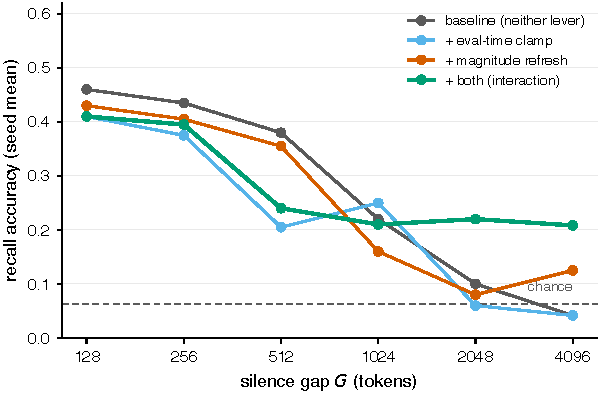
\includegraphics[width=4.60in]{fig_persistence_knee.pdf}
\caption{The persistence knee moves with the eval-time levers. Each lever
alone decays toward chance beyond $G{\approx}512$--$1024$; applying both
together holds recall at more than $3{\times}$ chance out to $G{=}4096$
--- an interaction, not a sum. Source:
\code{results/holo\_clamp\_refresh.json}.}
\label{fig:knee}
\end{figure}

\paragraph{F4 --- The two-system law.} The gated-readout cliff
(rank-1-per-channel binding, $D_\text{eff} \approx 1.02$ measured against a
closed-form bound) forces unbounded accumulation into an external index.
Runtime consultation lifts recall far past state capacity (0.10--0.20
$\to$ 0.41--0.62 at 16 pairs, dose-dependent, random-injection controlled);
models trained \emph{with} consultation read reminders at 0.99--1.00.

\paragraph{F5 --- Family-generic operating modes.} The full POS recipe run
on a scan-parameter-matched Mamba/S6 configuration transfers at
0.98$\times$ (three seeds, two CPU architectures) --- and the house operator
beats S6 head-to-head (+0.13 to +0.16 nats) at parity. The calculus attaches
to the operator class, not to one network.

\paragraph{F6 --- Train short, deploy unbounded.} One shift-equivariance
symmetry on two axes: sequence length (flat to $4096\times$; corpus-as-
iterator to $10^9$ tokens) and silence (keyed bindings held through gaps
$128\times$ the training horizon). Its honest boundary is measured twice:
multi-chunk training is structurally gradient-blind to the write --- the
cure is to train inside the boundary and let exactness carry the skill out.

\paragraph{F7 --- The portable organism.} The complete living system ---
weights, optimizer moments, carried state, gating windows, span store,
stream position, RNG --- is one atomic $\sim$53~MB artifact, and the organs
couple through \emph{kilobytes} (spans, reminders, deltas), not activations.
Measured: local checkpoint$\to$new-process$\to$resume is bit-identical;
\textbf{live mid-stream migration from Apple Silicon to x86 continues
behaviorally identically to six decimals} (heldout 6.182391 == 6.182391,
every gate decision matched --- only the BLAS bit-digest differs, and it
does not propagate); a killed replica rejoining through a \emph{shared} span
store ends \emph{better} than its never-killed twin ($-0.014$: the
partner's outage-window spans are a gift); an outage spent sleeping beats
one spent idle (+0.065); stop-free migration (source never pauses, target
catches up by deterministic replay) achieves bit-identical parity at every
scale tried.

\section{The 40-hour experiment: the gate beats the firehose}
\label{sec:40h}

One process, three from-scratch arms on one cloned C4 stream (seed 42), 40.0
hours, 909{,}676{,}544 tokens, no restarts, RSS $\le$ 1.094~GB. A1: forward
only. A2: backward on every chunk. A3: backward only when the chunk's own
mean NLL clears the rolling 75th percentile of its own history --- no
oracle, no second model, no labels, no schedule.

\begin{table}[h]
\centering
\caption{The 40-hour surprise-gated run vs.\ full-gradient training.}
\label{tab:40h}
\begin{tabular}{@{}lccc@{}}
\toprule
arm & held-out $8.6588 \to$ & improvement & gradient tokens\\
\midrule
A2 full-gradient & 4.7782 & 3.8806 & 100\%\\
\textbf{A3 surprise-gated} & \textbf{4.7430} & \textbf{3.9158} & \textbf{25.17\%}\\
\bottomrule
\end{tabular}
\end{table}

\textbf{Ratio 1.0091.} The pre-registered prediction (P1) put the point
estimate at 0.85 with an explicit embarrassment threshold: \emph{``ratio
$>$ 1.0 sustained would be a bigger result than the thesis itself.''} It
fired. The surprising part is not efficiency --- it is that the 75\% of
chunks the gate skips are, in net, \emph{worth skipping}: selective
plasticity beats indiscriminate plasticity at equal data exposure. Every
number re-derives from the raw 1.78M-chunk log (16/16 integrity checks).

\begin{figure}[t]
\centering
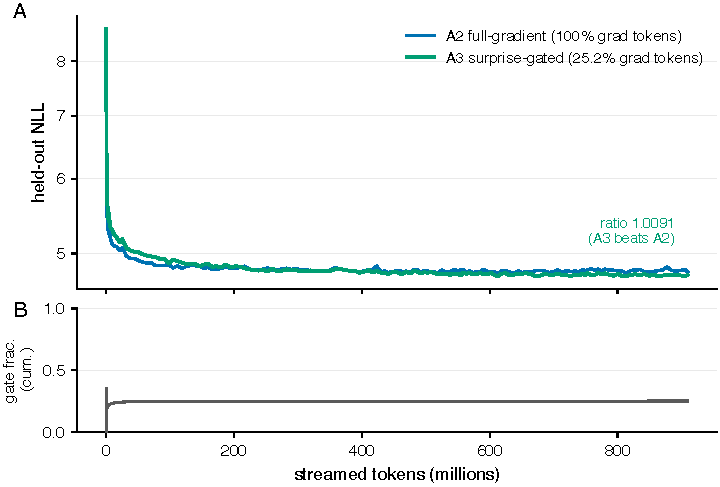
\includegraphics[width=5.50in]{fig_40h_gate_beats_firehose.pdf}
\caption{The 40-hour run: held-out loss for A2 (full-gradient) and A3
(surprise-gated), and A3's cumulative gate fraction, vs.\ streamed tokens.
A3 tracks A2 while training on 25.2\% of the gradient tokens and finishes
ahead (ratio 1.0091). Source: \code{results/pos\_metrics.jsonl}.}
\label{fig:40h}
\end{figure}

\textbf{The twin.} At T+24h, A3's weights were copied into a fresh process
with zero carried state. Registered: a warmup tax (+0.03--0.15 excess
surprise, $\ge 1.5\times$ over-gating, hours to converge). Measured: excess
0.0029, gate rates identical to four decimals, convergence one chunk after
the fork, and the twin finished \emph{ahead} (4.7365). Restarting a living
stream is free at the fast timescale --- the third independent measurement
of the two-timescale law (\S\ref{sec:twotimescale}).

\begin{figure}[t]
\centering
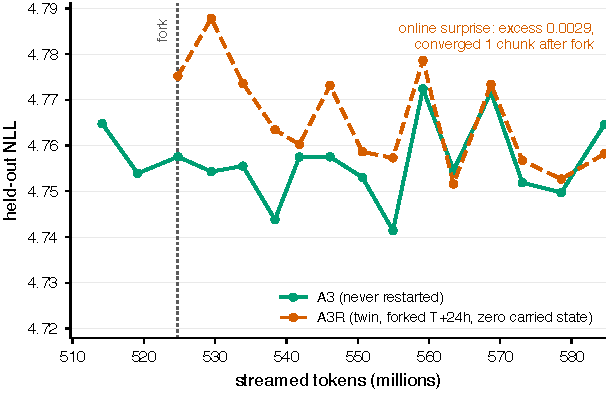
\includegraphics[width=4.60in]{fig_twin_recovery.pdf}
\caption{The twin, zoomed to the fork. A3R (forked at T+24h with zero
carried state) opens ${\approx}0.02$ nats above A3, crosses into A3's own
fluctuation band within a few evaluations, and finishes ahead (4.7365
vs.\ 4.7430). On the registered online-surprise criterion the restart is
free: excess 0.0029, gate fractions identical to four decimals,
convergence one chunk after the fork. Source:
\code{results/pos\_metrics.jsonl}, \code{results/pos\_summary.json}.}
\label{fig:twin}
\end{figure}

\textbf{The honest negative.} 1020 paired index-injection probes: both
deltas negative (the index froze at its 20k cap by token 11M; replaying
5--11M-era spans into an $80\times$-older model disturbs), but injection
hurts $3.2\times$ \emph{less} than random injection ($-0.087$ vs.\ $-0.279$;
helped 0.35 vs.\ 0.10) --- the mechanism carries information; the
provenance was stale. Registered as falsified; the v2 (rolling spike
threshold) is specified.

\section{The two-timescale law of operation}
\label{sec:twotimescale}

Three independent experiments give the same law. (1) The twin
(\S\ref{sec:40h}): zero carried state costs nothing. (2) A snapshot
cross-matrix (weights at 359M tokens $\times$ states from
128M/240M/359M/zero/shuffled): every arm converges to the native trajectory
within 4 chunks --- 256 tokens, the receptive-field scale; a cold start is
not worse than the carried state. (3) The beacon: a \emph{stored bit} in a
write-once-freeze carrier channel ($\gamma \approx 0.9995$) survives a
d64$\to$d128 widening surgery at recall 1.000 and survives a weight swap
across $2\times$ training distance at recall 1.000 through 512 tokens of
silence --- by redundant encoding (the carrier's channel address can
relocate; the read still lands).

\textbf{The law:} the fast path forgets by design --- so weight updates,
model growth (function-preserving widening: surgery equivalence 6.7e-6, no
transient, growth beats restart by +0.13 to +0.17 nats, $3\times$
replicated), and migration are \emph{safe live operations}; everything
durable lives in slow carriers, weights, and the index --- exactly the
layer the organism's own calculus (F1, F4) manages. Operationally this is
the answer to a question every persistent-model deployment will face:
\emph{what must be preserved across an update?} Measured: almost nothing ---
if the architecture separates its timescales.

\section{The organism is social and collective}

Organism A streams a C4+code mix, storing its surprise spans. Organism B,
facing a code shock, replays A's shared spans and forgets \textbf{0.67$\times$}
of what it forgets with only its own spans --- at better plasticity ---
while token-shuffled A-spans are as useless as no replay: the benefit is
content, not regularization. Combined with F7: a fleet of small organisms
sharing an index is a \emph{measured} design, not an aspiration --- including
the striking corollary that a replica which dies and rejoins through the
shared store can end \emph{better} than one that never died.

\section{Method as contribution: the adversarial ledger}

Every experiment in this program was preceded by a numbered, committed
prediction (P1--P39 at this writing); a scoring script audits result JSONs
against the register; falsified predictions remain in the ledger with the
numbers that killed them. Of the scored predictions, roughly one third were
falsified or partial --- including the program's own favorite hypotheses
(the dream generator; rate-homeostatic curiosity; the $\alpha$-regularizer;
a one-parameter rent law; the phase advantage on real text --- falsified
\emph{and then explained} by a 16-cell rent map measured the same night,
Figure~\ref{fig:rent}).

\begin{figure}[t]
\centering
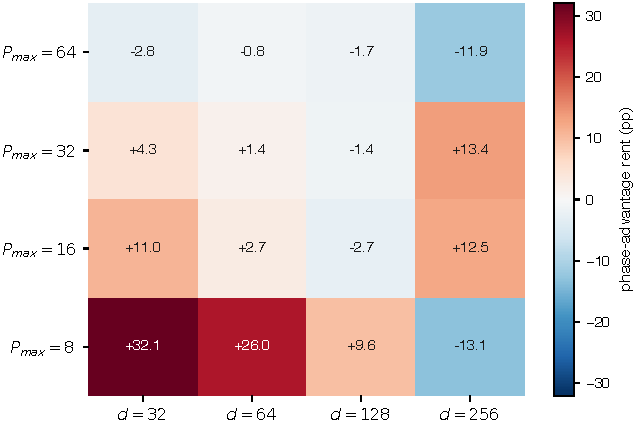
\includegraphics[width=4.20in]{fig_rent_map.pdf}
\caption{The 16-cell rent map: phase-advantage rent (percentage points) as
a function of the recall load $P_\text{max}$ and width $d_\text{model}$.
The one-parameter rent law that motivated a single scalar prediction is
falsified by this map's structure; the map explains, cell by cell, where
the phase advantage on real text holds and where it does not. Source:
\code{results/holo\_rent\_map.json}.}
\label{fig:rent}
\end{figure}
Two method-level findings emerged from the discipline itself:
\textbf{training-dynamics sensitivity to floating-point reduction order near
ignition boundaries} (thread count changes \emph{whether} a model ignites,
not just speed --- 6/6 seeds ignite in one regime, 0/4 in another), and the
resulting rule that instruments must reproduce their reference regime. We
offer the ledger pattern itself as a transferable practice: a vision paper
whose every claim is either a committed measurement or an explicitly open
registered question.

\section{The reality prediction engine (the road this opens)}

The foundations compose into something none of them states alone. A system
that (i) lives indefinitely on present streams at constant memory (F2, F6),
(ii) controls all plasticity from its own prediction error (F1) --- in the
spirit of temporal-difference learning's use of prediction error as a
teaching signal \cite{sutton1988td} and predictive coding's use of
prediction error as the currency of cortical inference \cite{rao1999predictive},
(iii) can \emph{deposit} a prediction about its own future in a persistence
mechanism built for exactly that (F3's carrier; measured to survive
silence, surgery, and weight updates) --- the world-model commitment
articulated for autonomous machine intelligence \cite{lecun2022path}, (iv)
scores the deposit when the future arrives --- a loop only a \emph{living}
system can close, because a batch model never experiences its own future
--- and (v) exists as a portable, forkable, shardable, collectively-
remembering asset (F7, \S 6): this is a \textbf{reality prediction engine}.
Its scaling axis is not parameters but \emph{scope} --- more streams, more
horizons, more organisms sharing more index. The first horizon-ladder
experiment (early-warning under distribution shift; the long-horizon head
as gating teacher) is registered (P37) and running at this draft's commit.

\section{Limitations, stated plainly}

Scale: $d_\text{model} \le 128$, WT-2-derived vocabularies; no claim of
frontier language quality is made or implied. The phase mechanism's
ignition is fragile (seed- and reduction-order-dependent) --- a measured
fact that bounds current practice and is itself a finding. The injection
result is provenance-limited (stale index era). Wall-clock throughput
numbers are never claimed (host contamination); all axes are token-based.
The rank-1 anchor's generating script is lost (artifact-backed,
reconstruction leads documented) --- reported as reproduction debt.

\section{Invitation}

Everything here reruns from the repository: the harnesses, the exact
configurations, the raw JSONs, the ledger, and the scoring script. The
organism that produced \S\ref{sec:40h} can be resumed, forked, migrated, or
extended by anyone --- that is what F7 is for.

\bigskip
\noindent\textit{Related work (to be expanded in v0.2): predictive coding
and JEPA (the vision lineage) \cite{rao1999predictive,lecun2022path},
TD-learning (multi-horizon error) \cite{sutton1988td}, zoology/MQAR (recall
instruments) \cite{arora2024zoology}, Mamba/S5/LRU (the operator family)
\cite{gu2023mamba,smith2023s5,orvieto2023lru}, VM live migration (the
systems analogy) \cite{clark2005livemigration}.}

{\small
\bibliographystyle{plain}
\bibliography{o1state_refs}
}

\end{document}
